% !TEX root = ../ITGO.tex

\subsection*{Tension/compression spring design problem}


This problem was introduced by \cite{TC}, and the objective is the minimization of the weight of a tension/compression spring (Figure \ref{fig:TC}). The problem has three continuous design variables, being them the diameter of spring wire ($x_1 = D$), the diameter of spring mean coil ($x_2 = d$) and the number of active coils ($x_3 = P$). It is subject to three nonlinear and one linear inequality constraints. The objective function value at the known global optimum is $f(\bm{x}^*) = 0.01266523$.

\begin{figure}[h]
\begin{center}
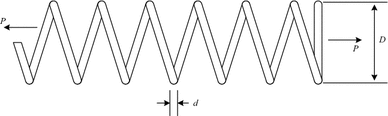
\includegraphics[scale=0.6]{Imgs/TC.png}
\end{center}
\captionsetup{justification=centering}
\caption{Schematic view of the tension/compression spring design problem.}\label{fig:TC}
\end{figure}


\prob{Appendix/Problems/TC}